%%%%%%%%%%%%%%%%%%%%%%%%%%%%%%%%%%%%%%
% Multiplicative domain poster
% Created by Nathaniel Johnston
% August 2009
% http://www.nathanieljohnston.com/2009/08/latex-poster-template/
%%%%%%%%%%%%%%%%%%%%%%%%%%%%%%%%%%%%%%

\documentclass[final]{beamer}
\usepackage[scale=1.24]{beamerposter}
\usepackage{graphicx}			% allows us to import images

%-----------------------------------------------------------
% Custom commands that I use frequently
%-----------------------------------------------------------

\newcommand{\bb}[1]{\mathbb{#1}}
\newcommand{\cl}[1]{\mathcal{#1}}
\newcommand{\fA}{\mathfrak{A}}
\newcommand{\fB}{\mathfrak{B}}
\newcommand{\Tr}{{\rm Tr}}
\newtheorem{thm}{Theorem}

%-----------------------------------------------------------
% Define the column width and poster size
% To set effective sepwid, onecolwid and twocolwid values, first choose how many columns you want and how much separation you want between columns
% The separation I chose is 0.024 and I want 4 columns
% Then set onecolwid to be (1-(4+1)*0.024)/4 = 0.22
% Set twocolwid to be 2*onecolwid + sepwid = 0.464
%-----------------------------------------------------------

\newlength{\sepwid}
\newlength{\onecolwid}
\newlength{\twocolwid}
\setlength{\paperwidth}{48in}
\setlength{\paperheight}{36in}
\setlength{\sepwid}{0.024\paperwidth}
\setlength{\onecolwid}{0.22\paperwidth}
\setlength{\twocolwid}{0.464\paperwidth}
\setlength{\topmargin}{-0.5in}
\usetheme{confposter}
\usepackage{exscale}

%-----------------------------------------------------------
% The next part fixes a problem with figure numbering. Thanks Nishan!
% When including a figure in your poster, be sure that the commands are typed in the following order:
% \begin{figure}
% \includegraphics[...]{...}
% \caption{...}
% \end{figure}
% That is, put the \caption after the \includegraphics
%-----------------------------------------------------------

\usecaptiontemplate{
\small
\structure{\insertcaptionname~\insertcaptionnumber:}
\insertcaption}

%-----------------------------------------------------------
% Define colours (see beamerthemeconfposter.sty to change these colour definitions)
%-----------------------------------------------------------

\setbeamercolor{block title}{fg=ngreen,bg=white}
\setbeamercolor{block body}{fg=black,bg=white}
\setbeamercolor{block alerted title}{fg=white,bg=dblue!70}
\setbeamercolor{block alerted body}{fg=black,bg=dblue!10}

%-----------------------------------------------------------
% Name and authors of poster/paper/research
%-----------------------------------------------------------

\title{Stability of Double Pulse Solutions to the 5th order Korteweg de Vries (KdV) Equation, a Numerical Approach}
\author{Ross Parker, Bj\"{o}rn Sandstede}
\institute{Division of Applied Mathematics, Brown University}

%-----------------------------------------------------------
% Start the poster itself
%-----------------------------------------------------------
% The \rmfamily command is used frequently throughout the poster to force a serif font to be used for the body text
% Serif font is better for small text, sans-serif font is better for headers (for readability reasons)
%-----------------------------------------------------------

\begin{document}
\begin{frame}[t]
  \begin{columns}[t]												% the [t] option aligns the column's content at the top
    \begin{column}{\sepwid}\end{column}			% empty spacer column

% first column
    \begin{column}{\onecolwid}
      \begin{alertblock}{Goal}
        \rmfamily{
        Examine the spectral stability of the linearization of the 5th order KdV equation about
        double pulse solutions.
        }
      \end{alertblock}

      \vskip1ex

      \begin{block}{Fifth-order KdV Equation}
        \rmfamily{
            \[ u_t = u_{xxxxx} - u_{xxx} + u u_x \]
          Applications
          \begin{itemize}
            \item Capillary gravity water waves
            \item Plasma waves
            \item Laser optics
          \end{itemize}
        }
      \end{block}

      \vskip1ex

      \begin{block}{Traveling Wave Solutions}
        \rmfamily{
          Traveling wave ansatz $u(x, t) = u(x - ct, t)$
            \[ u_t = u_{xxxxx} - u_{xxx} - c u_x + u u_x \]
          
          Equilibrium solution satisfies 5th order ODE 
            \[ u_{xxxxx} - u_{xxx} - c u_x + u u_x = 0 \]

          Since we seek solutions which decay to 0 at $\pm \infty$, 
          integrate once to get 4th order ODE 
            \[u_{xxxx} - u_{xx} - cu + u^2 = 0\]

          Equation is Hamiltonian with conserved quantity
          \[
            H = u_x u_{xxx} - \frac{1}{2}u_x^2 - \frac{1}{2}u_{xx}^2 + \frac{c}{2}u^2 - \frac{1}{3}u^3
          \]
        }
      \end{block}

      \vskip1ex

      \begin{block}{Homoclinic Orbits}
        \rmfamily{
          Linearization about zero solution
            \[v_{xxxx} - v_{xx} - c v = 0 \]
          Eigenvalues of linearization
          \vskip0.1ex
            \[ \lambda = \pm \sqrt{ \frac{1 \pm \sqrt{1 - 4c } }{ 2} } \]
          \vskip0.5ex
          2D stable manifold, 2D unstable manifold\\
          \vskip2ex
          \textbf{Theorem.} \emph{For $c>0$, a homoclinic orbit (single pulse solution) $u(x)$ exists which is smooth, even, and decays exponentially to 0 as $x \rightarrow \pm \infty.$}
        }
      \end{block}
 
    \end{column}

\begin{column}{\sepwid}\end{column}     % empty spacer column

% second column
    \begin{column}{\onecolwid}

      \begin{block}{Bifurcation}
      \rmfamily{
      At $c = 1/4$, eigenvalues of linearization about zero solution undergo a bifurcation.
        \begin{figure}
          \begin{center}
            \includegraphics[width=0.7\textwidth]{images/eigbifurcation}
            \caption{Eigenvalue bifurcation.}
            \label{fig:bifurcation}
          \end{center}
        \end{figure}
        For $c > 1/4$, $\lambda = \pm \alpha \pm \beta i$. Single pulse solution has tail oscillations with frequency $\beta$.
      \begin{figure}
          \begin{center}
            \includegraphics[width=0.7\textwidth]{images/singlepulsemagright.pdf}
            \caption{Oscillatory tail of single pulse solution.}
            \label{fig:singlepulsemagright}
          \end{center}
        \end{figure}
      }
      \end{block} 

      \vskip1ex

      \begin{block}{Double Pulses}
      \rmfamily{
        Construct double pulse by joining single pulses at the critical points or zeros of tail oscillations.\\
        \vskip2ex
        \textbf{Theorem.} \emph{For $c>1/4$, a countably infinite family of double pulses exists, indexed by $n \in \mathbb{N}$. Double pulses resemble two copies of the single pulse separated by small-amplitude oscillatory tails. Distance between peaks is of order $n \pi / \beta.$
        }
      }
      \end{block}

      \vskip1ex

       \begin{block}{Numerical Methods}
        \rmfamily{
          \begin{itemize}
            \item Discretization schemes: Fourier and Chebyshev polynomial spectral methods
            \item Start with known solution for $c = \sqrt{6/13}$
            \item Parameter continuation in $c$ until $c > 1/4$
            \item Join two single pulses end-to-end at critical point or zero of tail oscillations
            \item Use Matlab's \texttt{fsolve} to solve 4th order ODE
          \end{itemize}
        }
      \end{block} 

    \end{column}

\begin{column}{\sepwid}\end{column}     % empty spacer column

% third column
    \begin{column}{\onecolwid}

      \begin{block}{Double Pulse Construction}
        \rmfamily{
          \begin{figure}
          \begin{center}
            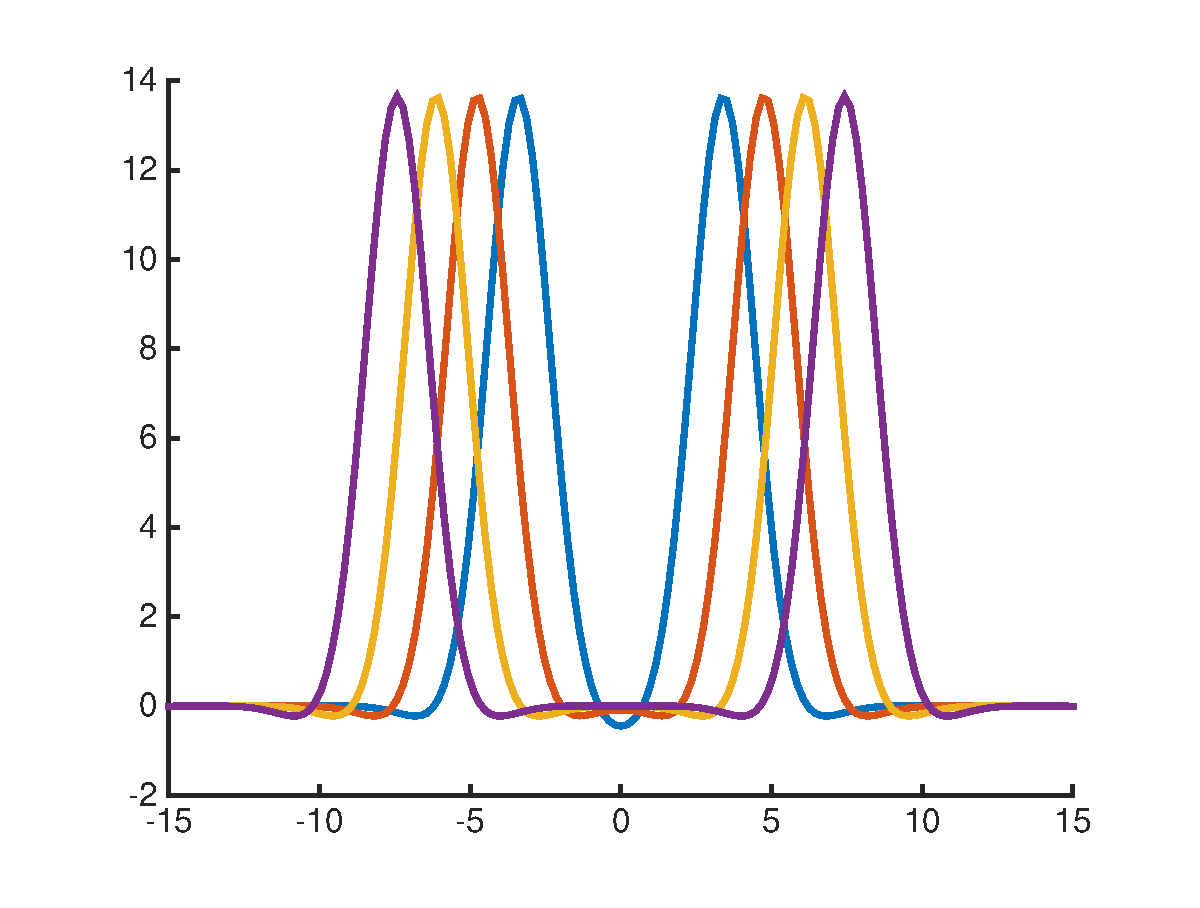
\includegraphics[width=0.7\textwidth]{images/doublepulses.eps}
            \caption{Double pulses 2(2), 2(3), 2(4), and 2(5).}
            \label{fig:doublepulses}
          \end{center}
          \end{figure}
        }
      \end{block} 

      \vskip1ex

      \begin{block}{Eigenvalues of Double Pulses}
        \rmfamily{
            \begin{itemize}
              \item Essential spectrum is entire imaginary axis
              \item Double eigenvalue at 0, eigenfunctions $\phi_x$ and $\phi_c$
              \item Additional eigenvalues near 0 from pulse interaction, Hamiltonian symmetry
            \end{itemize}

            \begin{figure}
              \begin{center}
              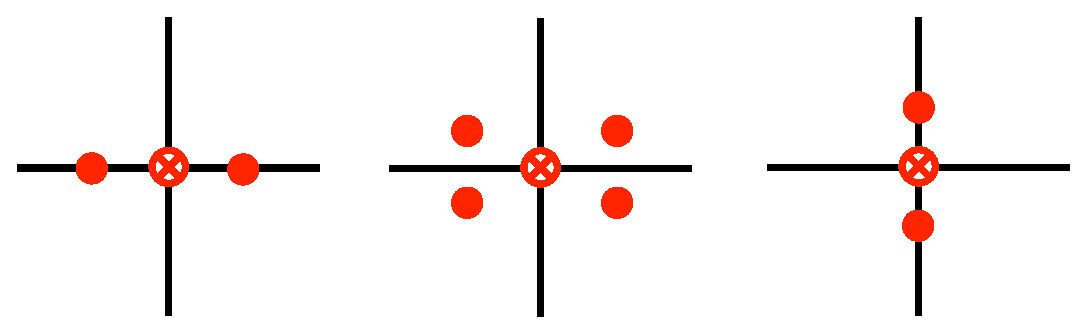
\includegraphics[width=0.8\textwidth]{images/eigdouble}
              \caption{Three possibilities for eigenvalues near 0.}
              \label{fig:eigcartoon}
            \end{center}
            \end{figure}

          Numerical computation using Matlab's \texttt{eig}.
          \begin{figure}
          \begin{center}
            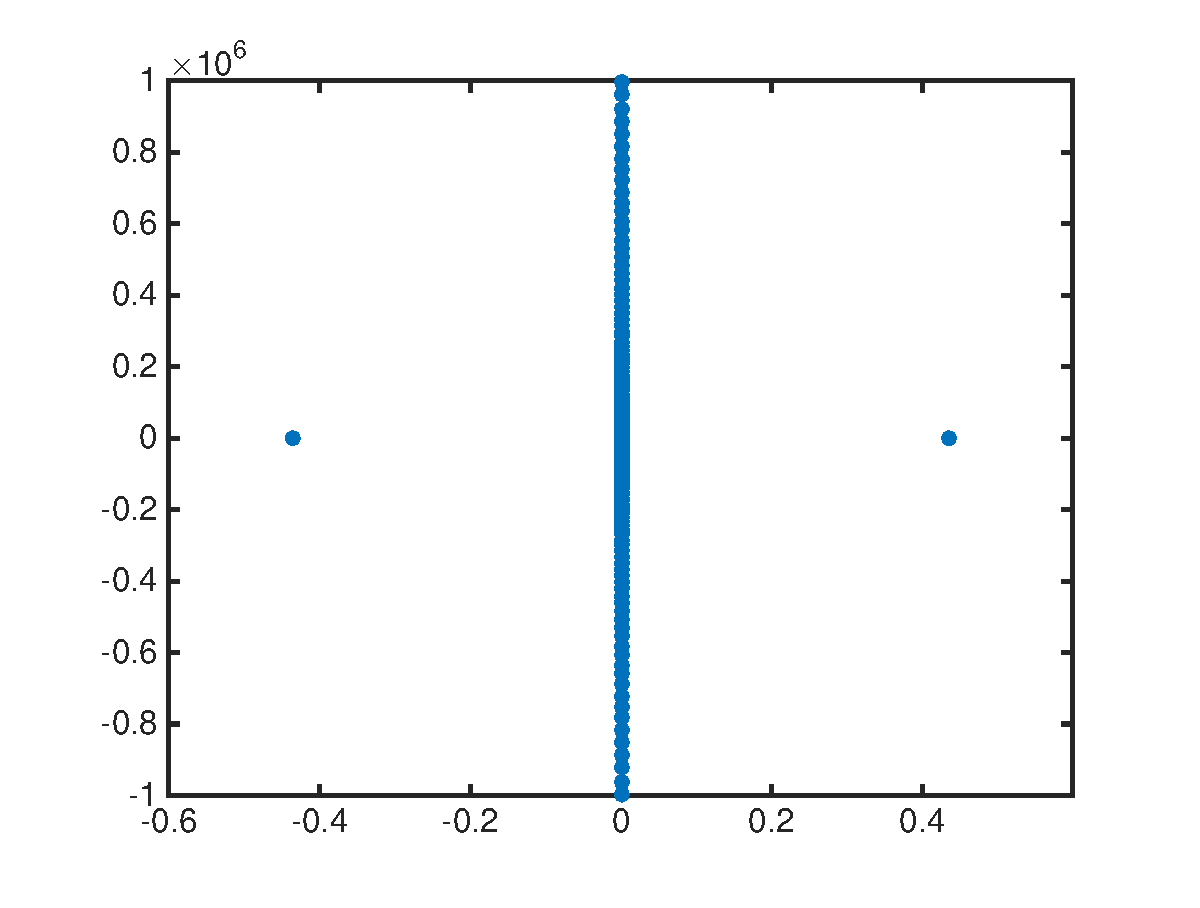
\includegraphics[width=0.5\textwidth]{images/unstableeig.eps}
            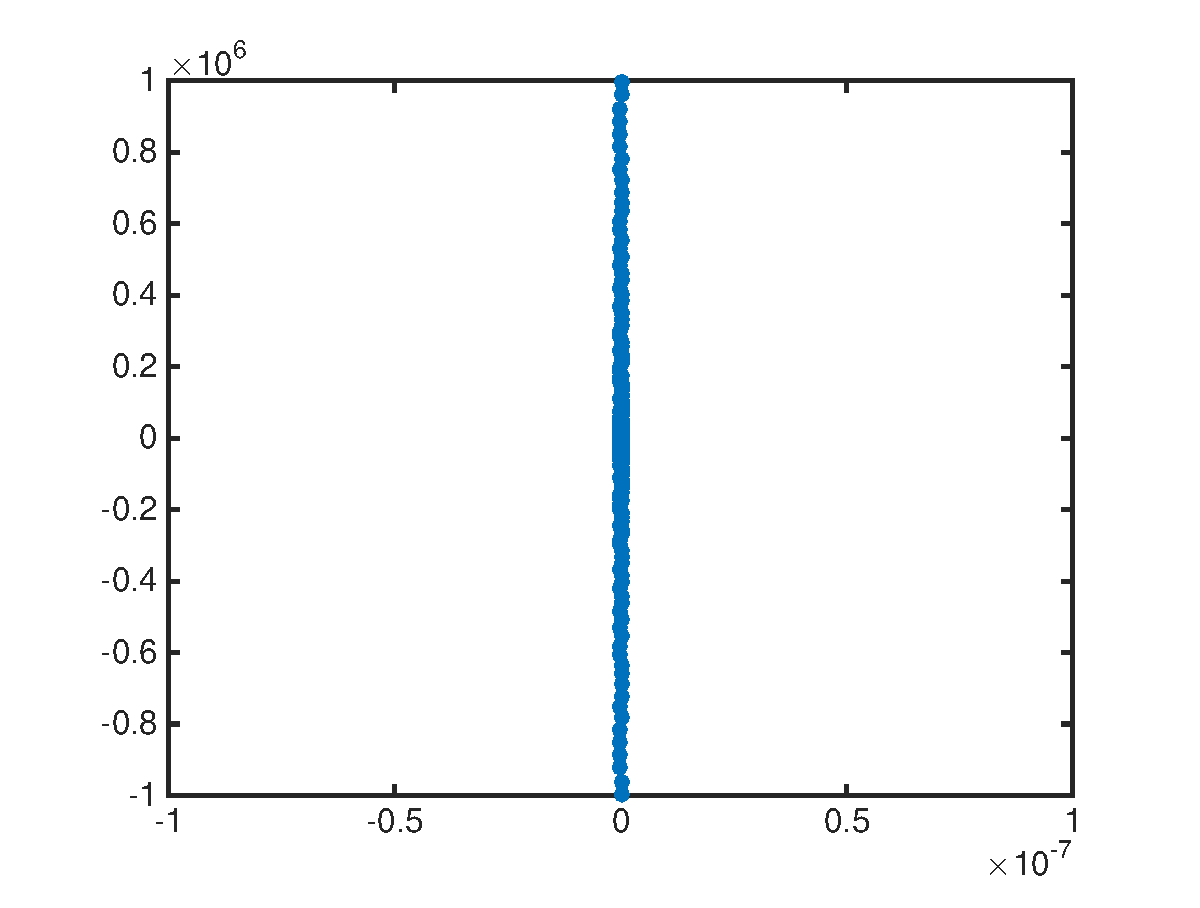
\includegraphics[width=0.5\textwidth]{images/stableeig.eps}
            \caption{Eigenvalues of linearization about double pulse 2(2) (left) and 2(3) (right).}
            \label{fig:numericaleig}
          \end{center}
          \end{figure}
        }
      \end{block} 

      \vskip1ex

      \begin{block}{Potentially Stable Double Pulses}
        \rmfamily{
          \begin{itemize}
            \item To find eigenvalues, use exponentially weighted space to move essential spectrum to the left
            \item For $c = 10$, we have a pair of eigenvalues at
            \[
            \lambda = 2.0829 \times 10^{-11} \pm 0.0691i
            \]
          \end{itemize}

        }
      \end{block} 

    \end{column}

  \begin{column}{\sepwid}\end{column}			% empty spacer column

  \begin{column}{\onecolwid}
    \begin{block}{Time Stepping}
      \rmfamily{
        \begin{itemize}
        \item  Chebyshev polynomial discretization in space
        \item Crank-Nicolson/Adams-Bashforth 2 IMEX scheme for time-stepping
      \end{itemize}
      \begin{figure}
        \begin{center}
          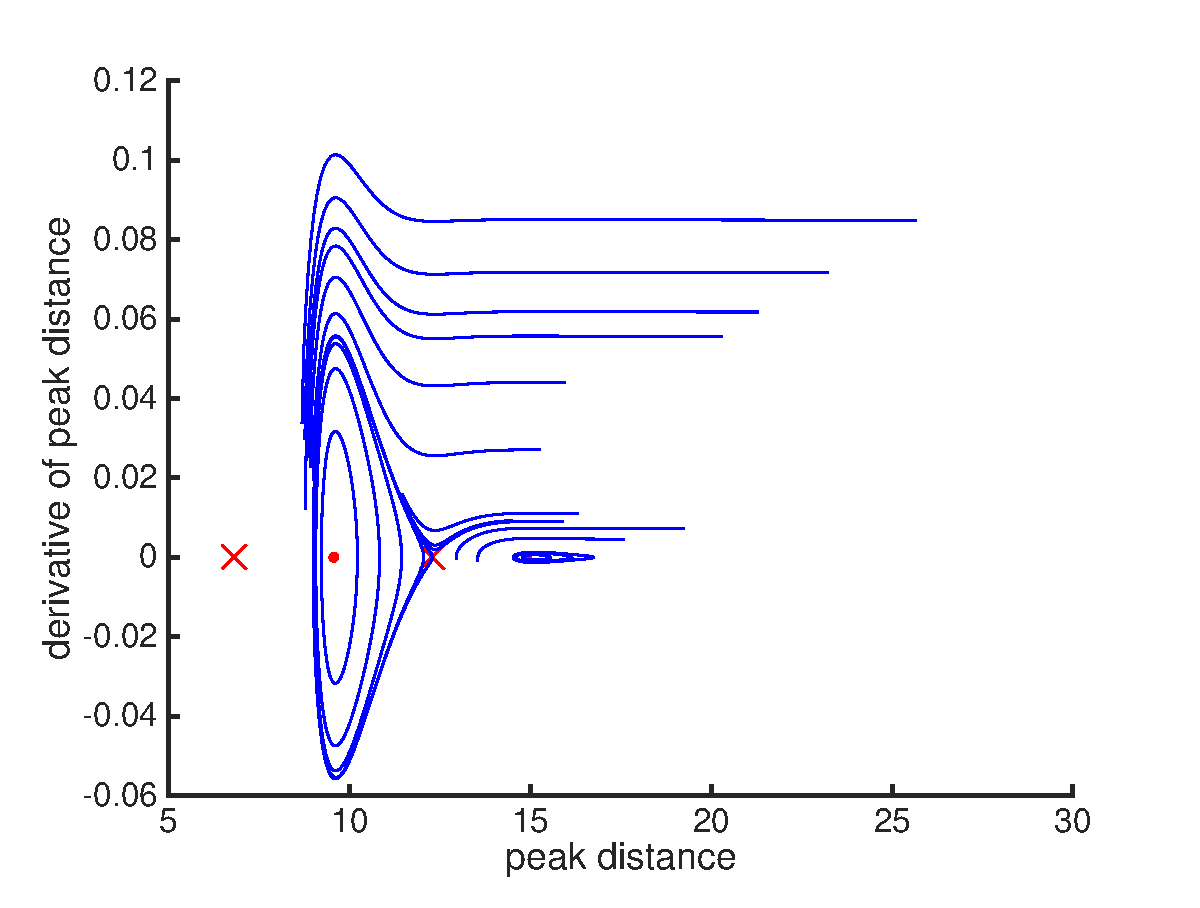
\includegraphics[width=0.8\linewidth]{images/phaseportrait3.eps}
            \caption{Derivative of peak distance versus peak distance.}
            \label{fig:timestep}
        \end{center}
      \end{figure}
      }
    \end{block}

    \vskip1ex

    \begin{block}{Future Work}
        \rmfamily{
        \begin{itemize}
          \item Prove that the eigenvalues of the potentially stable double pulse are pure imaginary to leading order in the pulse distance
          \item Prove spectral stability for the periodic case
          \item Examine stability of multipulse solutions for lattice PDEs
        \end{itemize}
        }
      \end{block} 

    \vskip1ex
  
    \begin{block}{References}
      \small{\rmfamily{\begin{thebibliography}{99}
      \bibitem{Buf}Buffoni B and S\'er\'e E. \emph{A global condition for quasi-random behaviour in a class of conservative systems}. Commun. Pure Appl. Math., 49 (1996), 285-305.
      \bibitem{Chug}Chugunova M and Pelinovsky P. \emph{Two-pulse solutions in the fifth-order KdV equation: Rigorous theory and numerical approximations}. Discrete and Continuous Dynamical Systems, Series B 8.4 (2007), 773-800.
      \bibitem{Grov}Groves M D. \emph{Solitary-wave solutions to a class of fifth-order model equations}. Nonlinearity, 11 (1998), 341-353.
      \bibitem{Sand} Sandstede B. \emph{Stability of multiple-pulse solutions}. Trans. Am. Math. Soc., 350 (1998), 429-472.
      \end{thebibliography}}}
    \end{block}

    \vskip1ex

    \begin{block}{Acknowledgments}
      \small{\rmfamily{This work is supported by the NSF Grant 1148284 }} \\
      \vspace{0.5in}
    \end{block}
  \end{column}
  \begin{column}{\sepwid}\end{column}			% empty spacer column
 \end{columns}
\end{frame}
\end{document}
